\documentclass{beamer}
\usepackage{color}
\usepackage{listings}
\usepackage{verbatim}
\usepackage{graphicx}
\usepackage{multicol}
\usepackage[utf8]{inputenc}
\usepackage{amsmath}
\usepackage{graphicx}
\usetheme{Madrid}
\title{Bachelor-Thesis Proposal}
\subtitle{Simulation of the RoboCup Logistic League with Fawkes and Gazebo for Multi-Robot Coordination Evaluation}
\author {Frederik Zwilling}
\institute{RWTH Aachen}
\date{23.07.13}
\subject{Multi-Robot Simulation}

\begin{document}
\frame{\titlepage}

%Übersicht
%\begin{frame}
%\frametitle{Overview}
%\begin{enumerate}
%\item Motivation
%\item Software Foundation
%\item Goals
%\item Conclusion
%\end{enumerate}
%\end{frame}

%Motivation
\begin{frame}
\frametitle{Motivation}
\begin{multicols}{2}
\begin{figure}
\only<1>{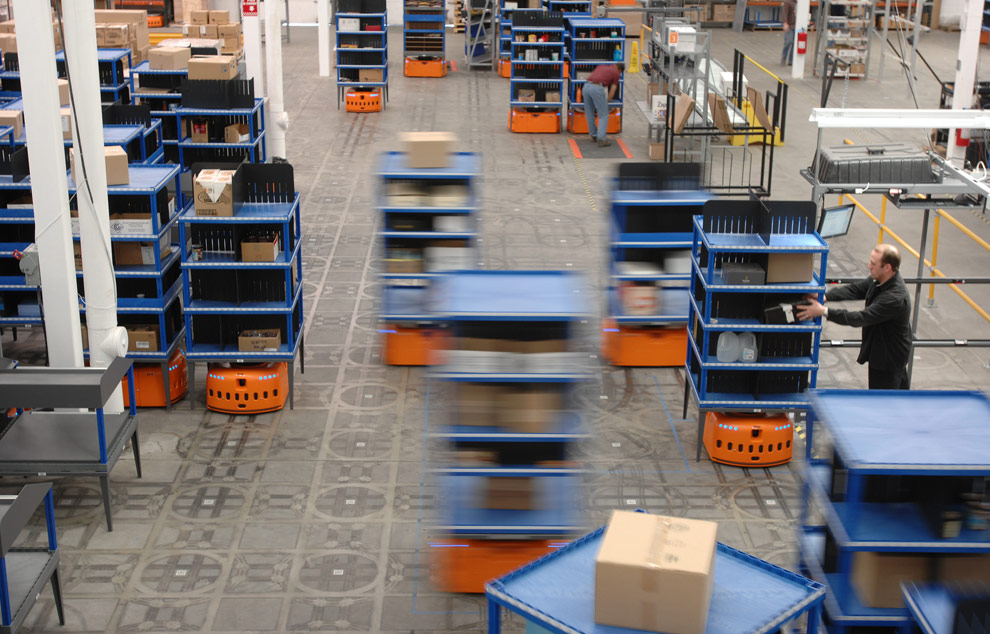
\includegraphics[width=140pt,heigth=100pt]{pics/kiva.jpg}\\}
\only<2>{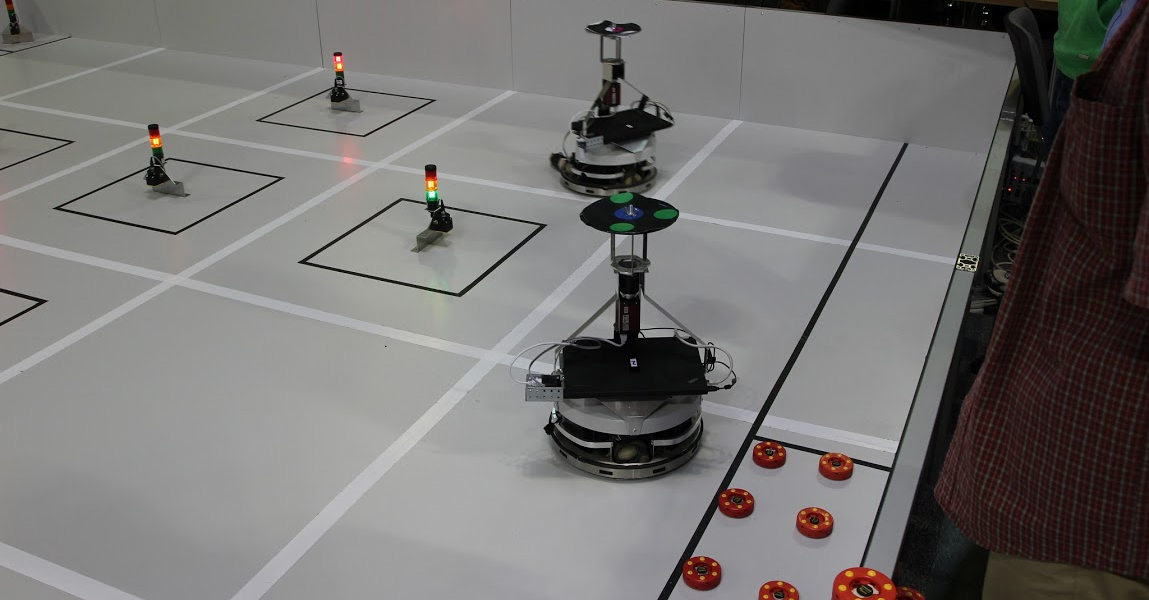
\includegraphics[width=140pt,heigth=100pt]{pics/llsf.jpg}\\}
\only<3->{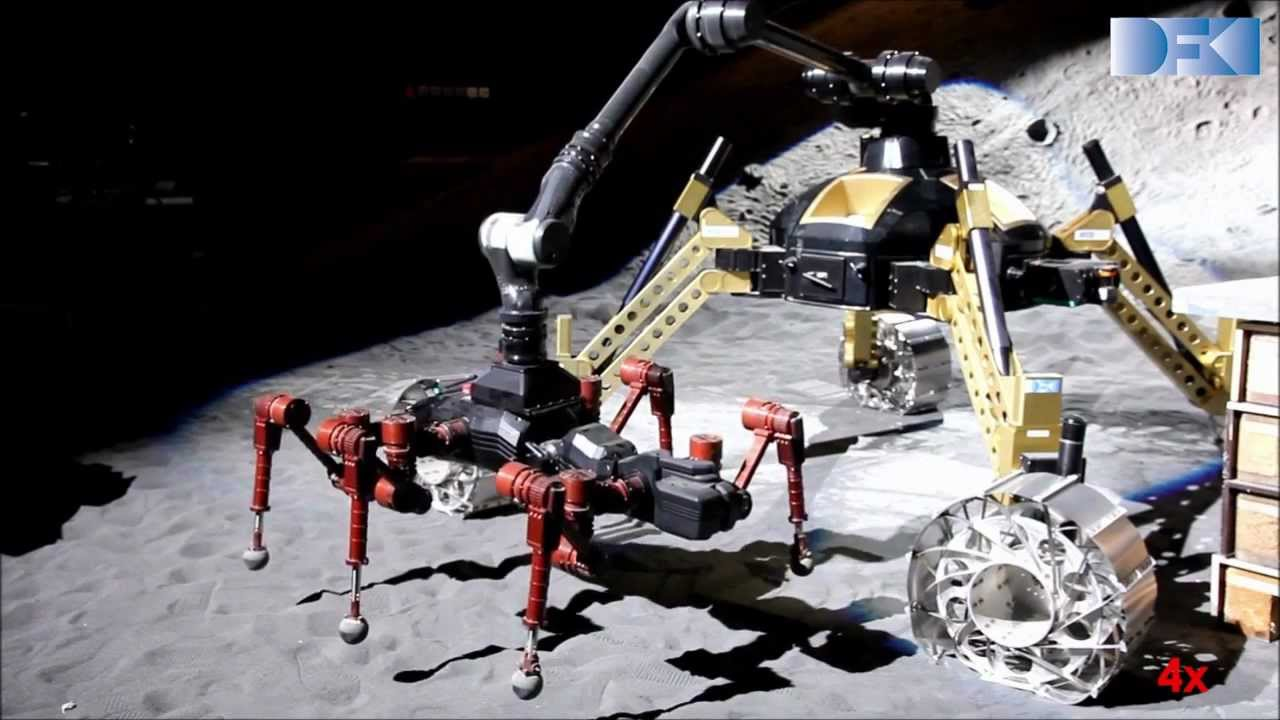
\includegraphics[width=140pt,heigth=100pt]{pics/rimes.jpg}\\}
\end{figure}
Fields with multi-robot systems:
\begin{itemize}
\item<1-> warehousing
\item<2-> logistics
\item<3-> many other domains
\end{itemize}
\end{multicols}
\pause \pause \pause 
\begin{itemize}
\item[$\Rightarrow$] Multi-robot systems are useful and about to get more important
\end{itemize}
\end{frame}

\begin{frame}
\frametitle{Problem-Solution}
\begin{multicols}{2}
Testing Problems:
\begin{itemize}
\item Need of environment and robots
\item Setup of the Robots %Effort scaleing with number of robots
\item Separately testing of high level components
%\item Effort scaling with the number of robots
\item Time-consuming comparison of multi-agent strategies 
\item[$\Rightarrow$] Testing is time and resource consuming
\end{itemize}
Advantages of a Simulator:
\begin{itemize}
\item Simulated environment and robots
\item Only setup of the software
\item Providing ground truth simulation
%\item Adding more robots more easily in the simulation
\item Simulation running over night or in parallel
\item[$\Rightarrow$] Simulation saves time and resources
\end{itemize}
\end{multicols}
\end{frame}

\begin{frame}
\frametitle{Logistic League sponsored by Festo (LLSF)}
\fboxsep=0pt
\noindent%
\begin{minipage}[]{0.48\linewidth}
\begin{figure}
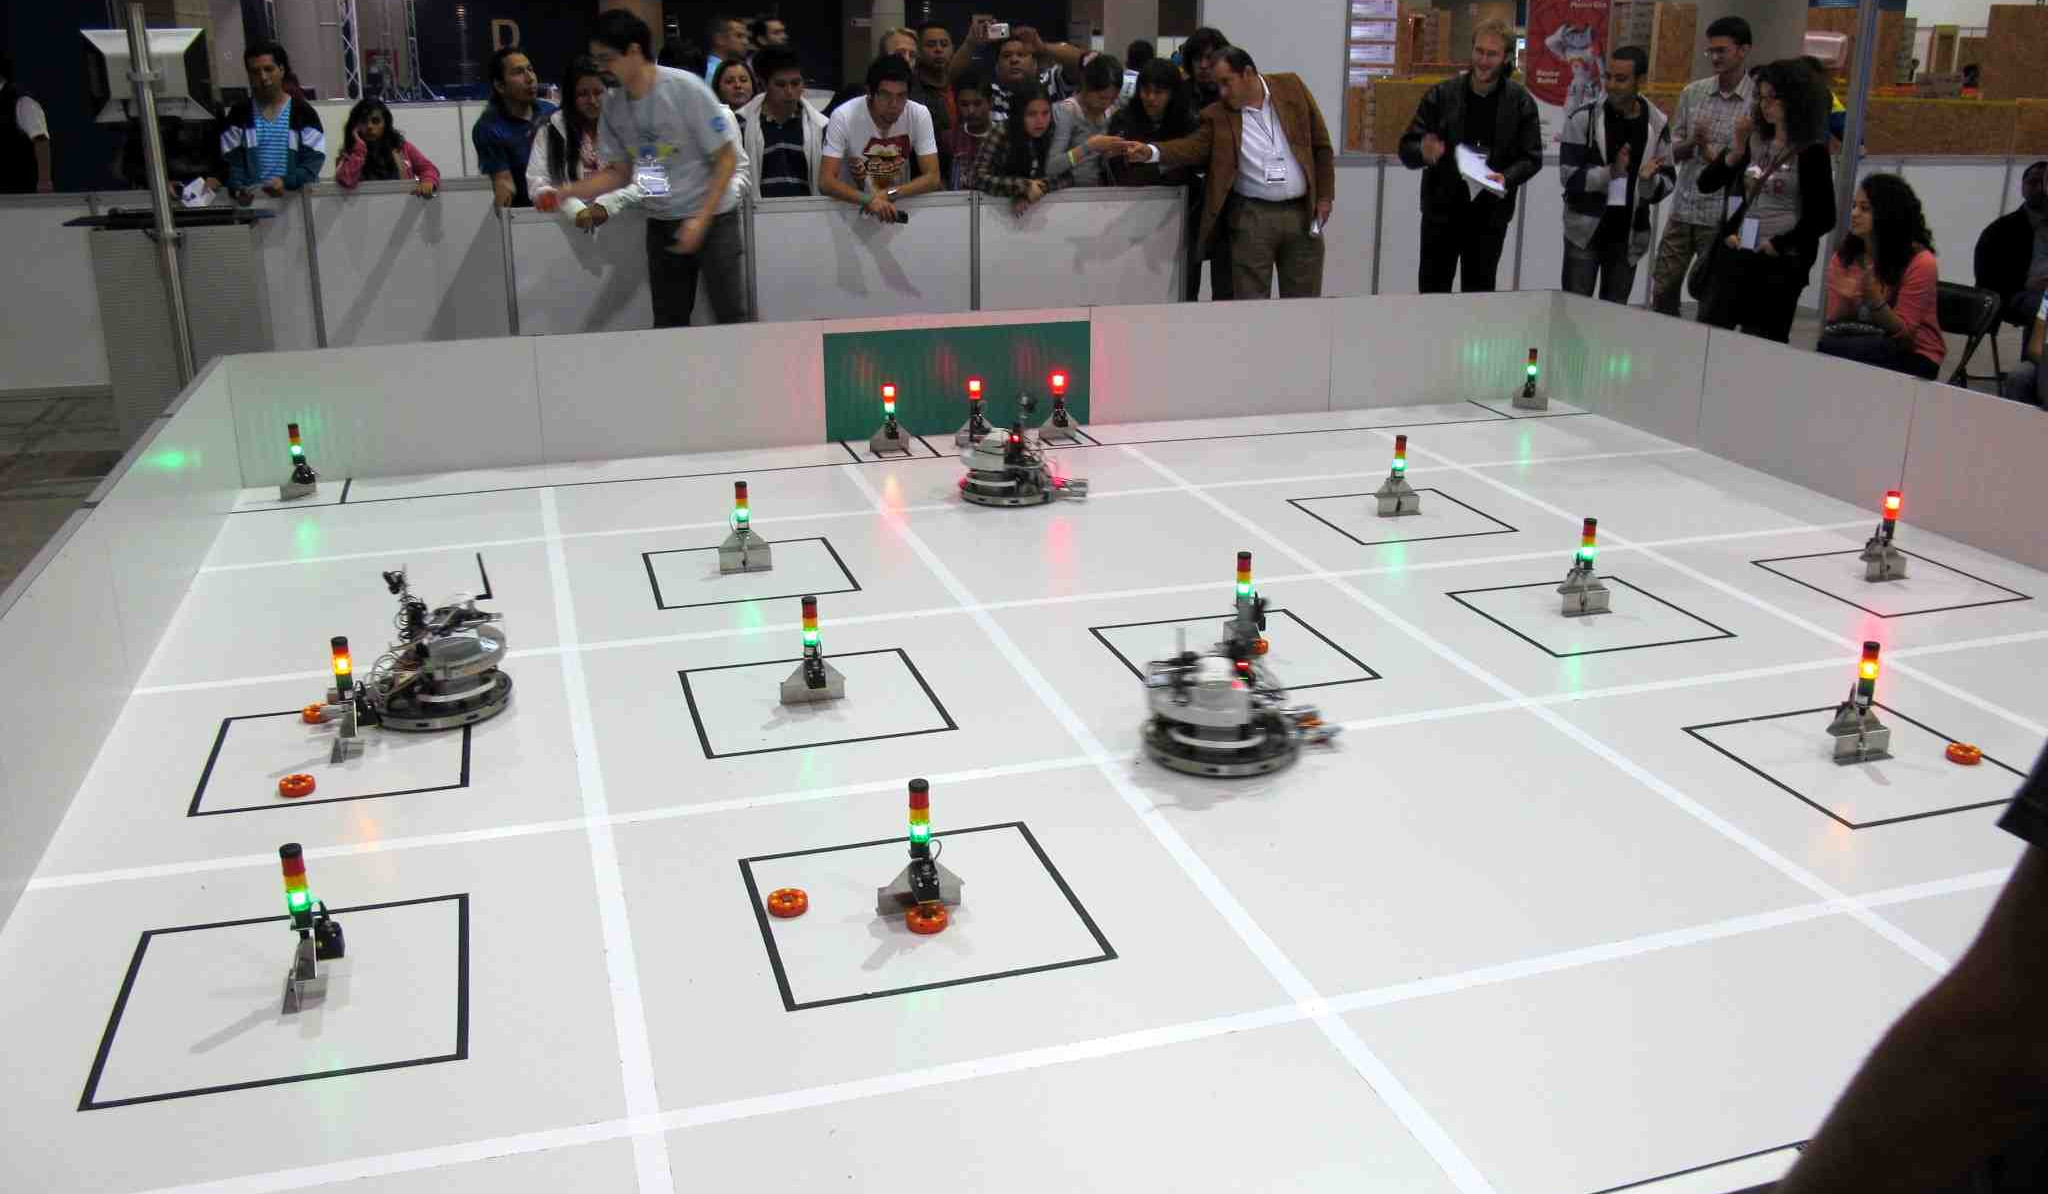
\includegraphics[width=150pt,heigth=120pt]{pics/llsfLeague.png}\\
\end{figure}
\end{minipage}%
\hfill%
\begin{minipage}[]{0.48\linewidth}
League:
\begin{itemize}
\item Part of RoboCup competition
\item Testbed for logistic robots in a competitive factory automation scenario
\end{itemize}
Task:
\begin{itemize}
\item Produce and deliver ordered products by feeding machines% with resources and semi-finished products
\item Optimize workflow and performance of the system
\end{itemize}
%Environment:
%\begin{itemize}
%\item Up to three Robotino robots
%\item 5.6m x 5.6m factory area
%\item Machines which indicate their state with light signals
%\item Pucks represent resources and products
%\end{itemize}
\end{minipage}
\end{frame}

\begin{frame}
\frametitle{Fawkes}
An Open Source robot software framework
\begin{itemize}
\item Developed and used primarily at KBSG
\item Component-based software design
\item Blackboard communication infrastructure\\ Plugins communicate through interfaces
\item[$\Rightarrow$] Easy exchange of sensor/actuator plugins by simulation plugins
\end{itemize}
\end{frame}

\begin{frame}
\frametitle{Gazebo}
\begin{multicols}{2}
An Open Source robot simulator
\begin{figure}
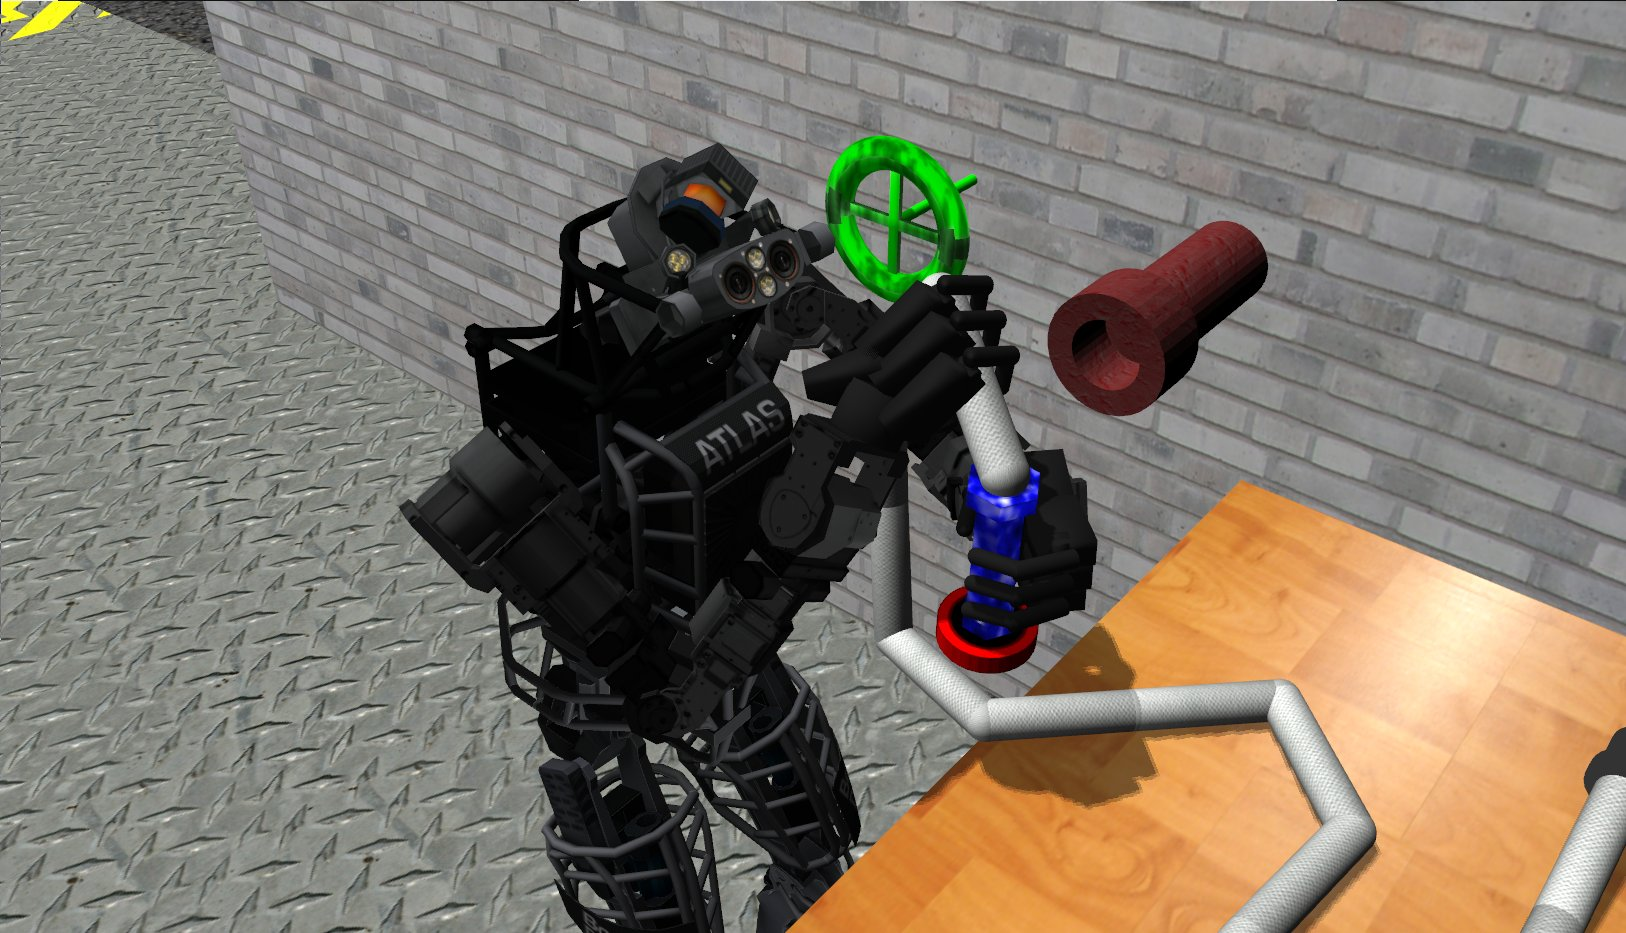
\includegraphics[scale=0.125]{pics/gazebo.jpg}
\end{figure}
\begin{itemize}
\item Ogre 3D Graphics Engine %Reflections
\item Open Dynamics Physics Engine %Slippery (Odom)
\item Plugin design approach
\item Already supports some robots and sensors %Hokujo
\item Highly founded
\end{itemize}
\end{multicols}
\begin{itemize}
\item[$\Rightarrow$] Suitable simulator for the thesis and future work
\end{itemize}
\end{frame}

\begin{frame}
\frametitle{Goals (1)}
Simulation environment for LLSF
\begin{itemize}
\item Communication Fawkes-Gazebo
\item Modeling the environment with behavior
%\item Implement machine behavior, rules, ...
\end{itemize}
Simulation of sensors and actuators
\begin{itemize}
\item High level simulation\\(e.g. provide ground truth, exact movement without collision)
\item Low level simulation\\(e.g. laser sensor data, movement by simulating the wheels)
\end{itemize}
\end{frame}

\begin{frame}
\frametitle{Goals (2)}
Multi-agent simulation
\begin{itemize}
\item Multiple robots in the simulation
\item Fawkes instance - simulated robot allocation
%\item Communication between agents
\end{itemize}
Expandability for future changes/extensions
\begin{itemize}
\item General interfaces between Fawkes and Gazebo
\item Modularity
\item Dokumentation
\end{itemize}
%Multi-level abstraction
%LLSF Challenges
\end{frame}

\begin{frame}
\frametitle{Multi-Agent Strategies, Evaluation}
Comparison of multi-agent strategies
\begin{itemize}
\item Current role-based approach vs. dynamic role allocation
\item Different roles of the third agent (e.g. production vs. recycling role)
\end{itemize}
Evaluation
\begin{itemize}
\item Qualitative\\(if and how well the simulation works)
\item Quantitative\\(resource usage, time difference, scalability)
\end{itemize}
\end{frame}

\begin{frame}
\frametitle{Conclusion}
\begin{itemize}
\item Multi-Robot Systems getting more important
\item Development/Testing difficult and time-consuming
\item[$\Rightarrow$] Simulation is a key to efficient development/testing
\item Goals: LLSF simulation, high/low level simulation, expabdability, comparison of multi-agent strategies
\item Short presentation of current state of development
\end{itemize}
\end{frame}


\end{document}
